\documentclass[tikz,border=10pt]{standalone}
\usepackage{amsmath}
\usetikzlibrary{arrows.meta, positioning, calc, decorations.pathreplacing}
\definecolor{c1}{HTML}{000000}
\definecolor{c2}{HTML}{233D4D}
\definecolor{c3}{HTML}{FE7F2D}
\definecolor{c4}{HTML}{EAECF0}
\definecolor{axiscolor}{HTML}{333333}
\definecolor{labelcolor}{HTML}{5F6B75}
\begin{document}
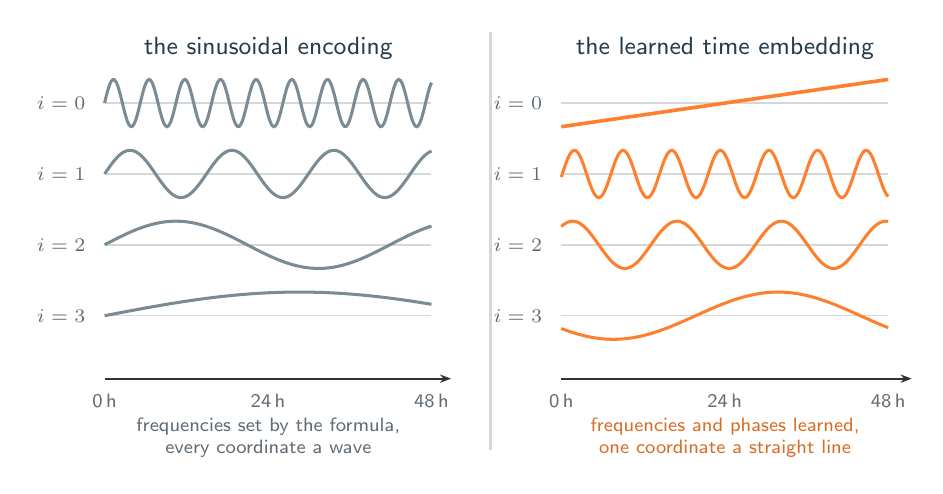
\begin{tikzpicture}[
    every node/.style={font=\sffamily},
    lab/.style={font=\sffamily\scriptsize, text=labelcolor},
    tag/.style={font=\sffamily\scriptsize, text=c2},
    hot/.style={font=\sffamily\scriptsize, text=c3!85!black},
]
\def\L#1{1.45 + #1*0.0865}
\def\R#1{7.25 + #1*0.0865}

\node[tag, font=\sffamily\small] at (3.53, 5.55) {the sinusoidal encoding};
\node[tag, font=\sffamily\small] at (9.33, 5.55) {the learned time embedding};
\draw[c2!20, line width=0.8pt] (6.35, 0.45) -- (6.35, 5.75);

% left: four coordinates, all waves, frequencies from the formula
\foreach \y/\w/\i in {4.85/1.20/0, 3.95/0.42/1, 3.05/0.15/2, 2.15/0.055/3}{
    \node[lab, anchor=east] at (1.33, \y) {$i = \i$};
    \draw[c2!20, line width=0.5pt] (1.45, \y) -- (5.60, \y);
    \draw[c2!60, line width=1.1pt]
        plot[domain=0:48, samples=200, smooth] ({\L{\x}}, {\y + 0.30*sin((\x*\w) r)});
}
\node[lab, anchor=north, align=center] at (3.53, 0.98)
    {frequencies set by the formula,\\ every coordinate a wave};

% right: one straight line plus learned waves
\node[lab, anchor=east] at (7.13, 4.85) {$i = 0$};
\draw[c2!20, line width=0.5pt] (7.25, 4.85) -- (11.40, 4.85);
\draw[c3, line width=1.3pt] ({\R{0}}, {4.85-0.30}) -- ({\R{48}}, {4.85+0.30});
\foreach \y/\w/\a/\i in {3.95/0.88/25/1, 3.05/0.41/70/2, 2.15/0.13/10/3}{
    \node[lab, anchor=east] at (7.13, \y) {$i = \i$};
    \draw[c2!20, line width=0.5pt] (7.25, \y) -- (11.40, \y);
    \draw[c3, line width=1.1pt]
        plot[domain=0:48, samples=200, smooth] ({\R{\x}}, {\y + 0.30*sin((\x*\w + \a) r)});
}
\node[hot, anchor=north, align=center] at (9.33, 0.98)
    {frequencies and phases learned,\\ one coordinate a straight line};

\draw[axiscolor, line width=0.7pt, -{Stealth[length=4pt]}] (1.45, 1.35) -- (5.85, 1.35);
\draw[axiscolor, line width=0.7pt, -{Stealth[length=4pt]}] (7.25, 1.35) -- (11.70, 1.35);
\foreach \p in {0, 24, 48}{
    \node[lab, anchor=north] at ({\L{\p}}, 1.28) {\p\,h};
    \node[lab, anchor=north] at ({\R{\p}}, 1.28) {\p\,h};
}

\end{tikzpicture}
\end{document}
